%%%%%%%%%%%%%%%%%%%%%%%%%%%%%%%%%%%%%%%%%%%%%%
\section{Introduction aux systèmes embarqués}
%%%%%%%%%%%%%%%%%%%%%%%%%%%%%%%%%%%%%%%%%%%%%%

\subsection{Systèmes embarqués}
\begin{frame}{Systèmes embarqués}
  \begin{itemize}
  \item Un système embarqué est un système concu pour ne réaliser qu'un certains nombre de tâches défini
  \item On associe un système à une fonction (ou un groupe de fonction)
  \item On cherche à maitriser le fonctionnement du système
  \item Différe des systèmes génériques censés savoir tout faire sur n'importe quelle plateforme
  \end{itemize}
\end{frame}

\begin{frame}{Exemples}
  \begin{tabular}{ccc}
    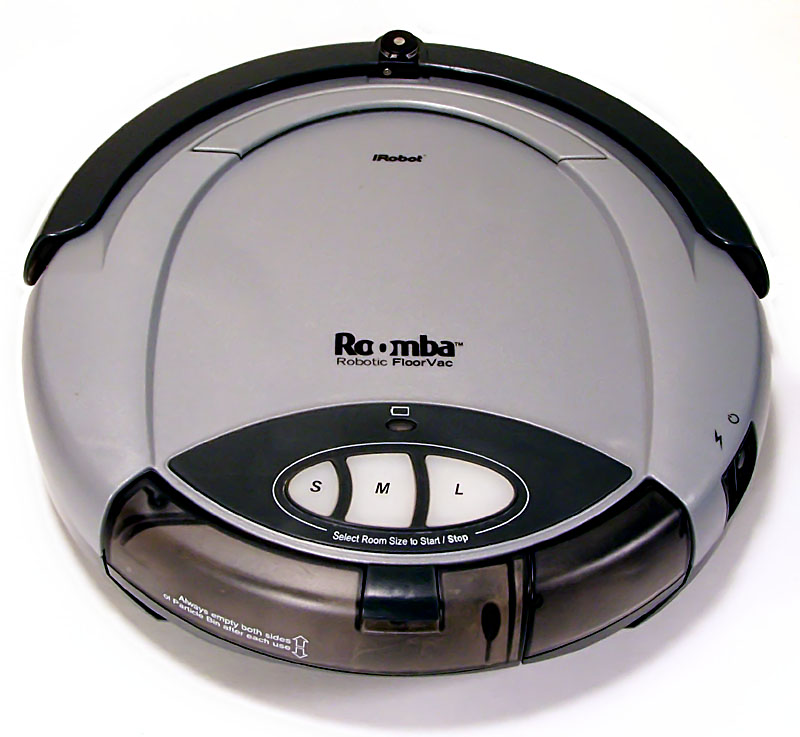
\includegraphics[height=2.5cm]{pictures/roomba.jpg} & \hspace{1.5cm}
    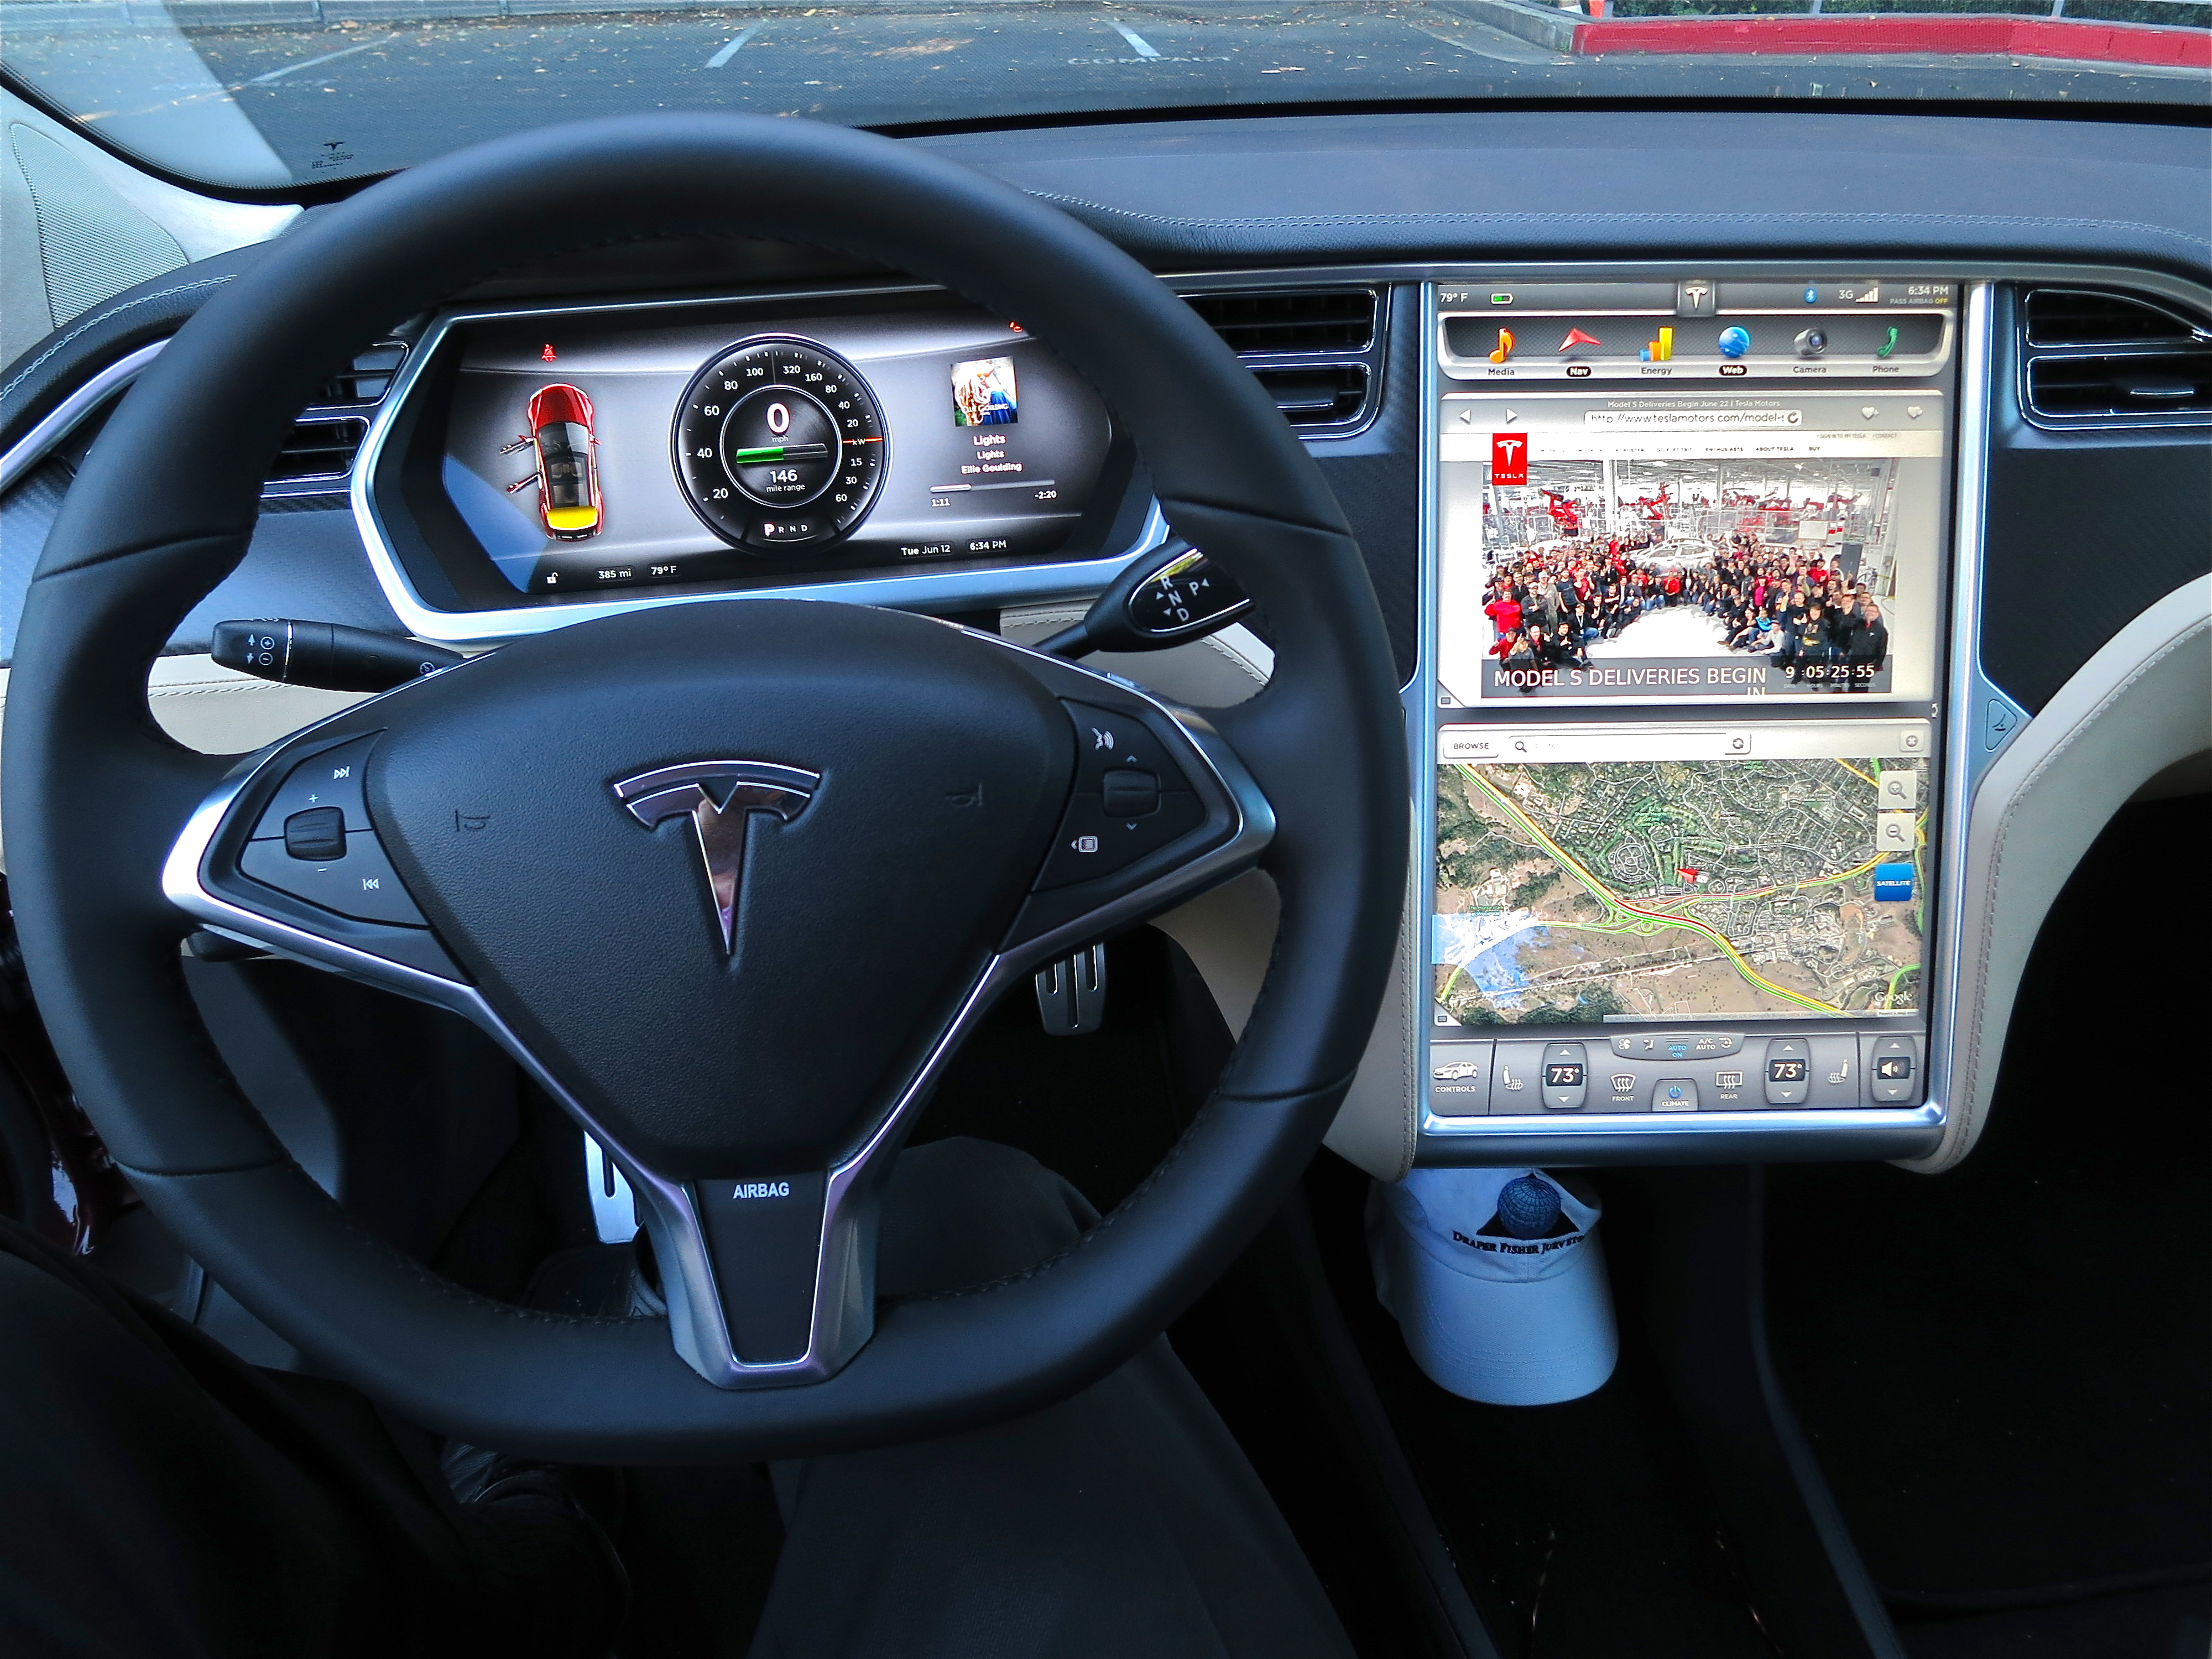
\includegraphics[height=2.5cm]{pictures/tesla.jpg} & \hspace{1.5cm}
    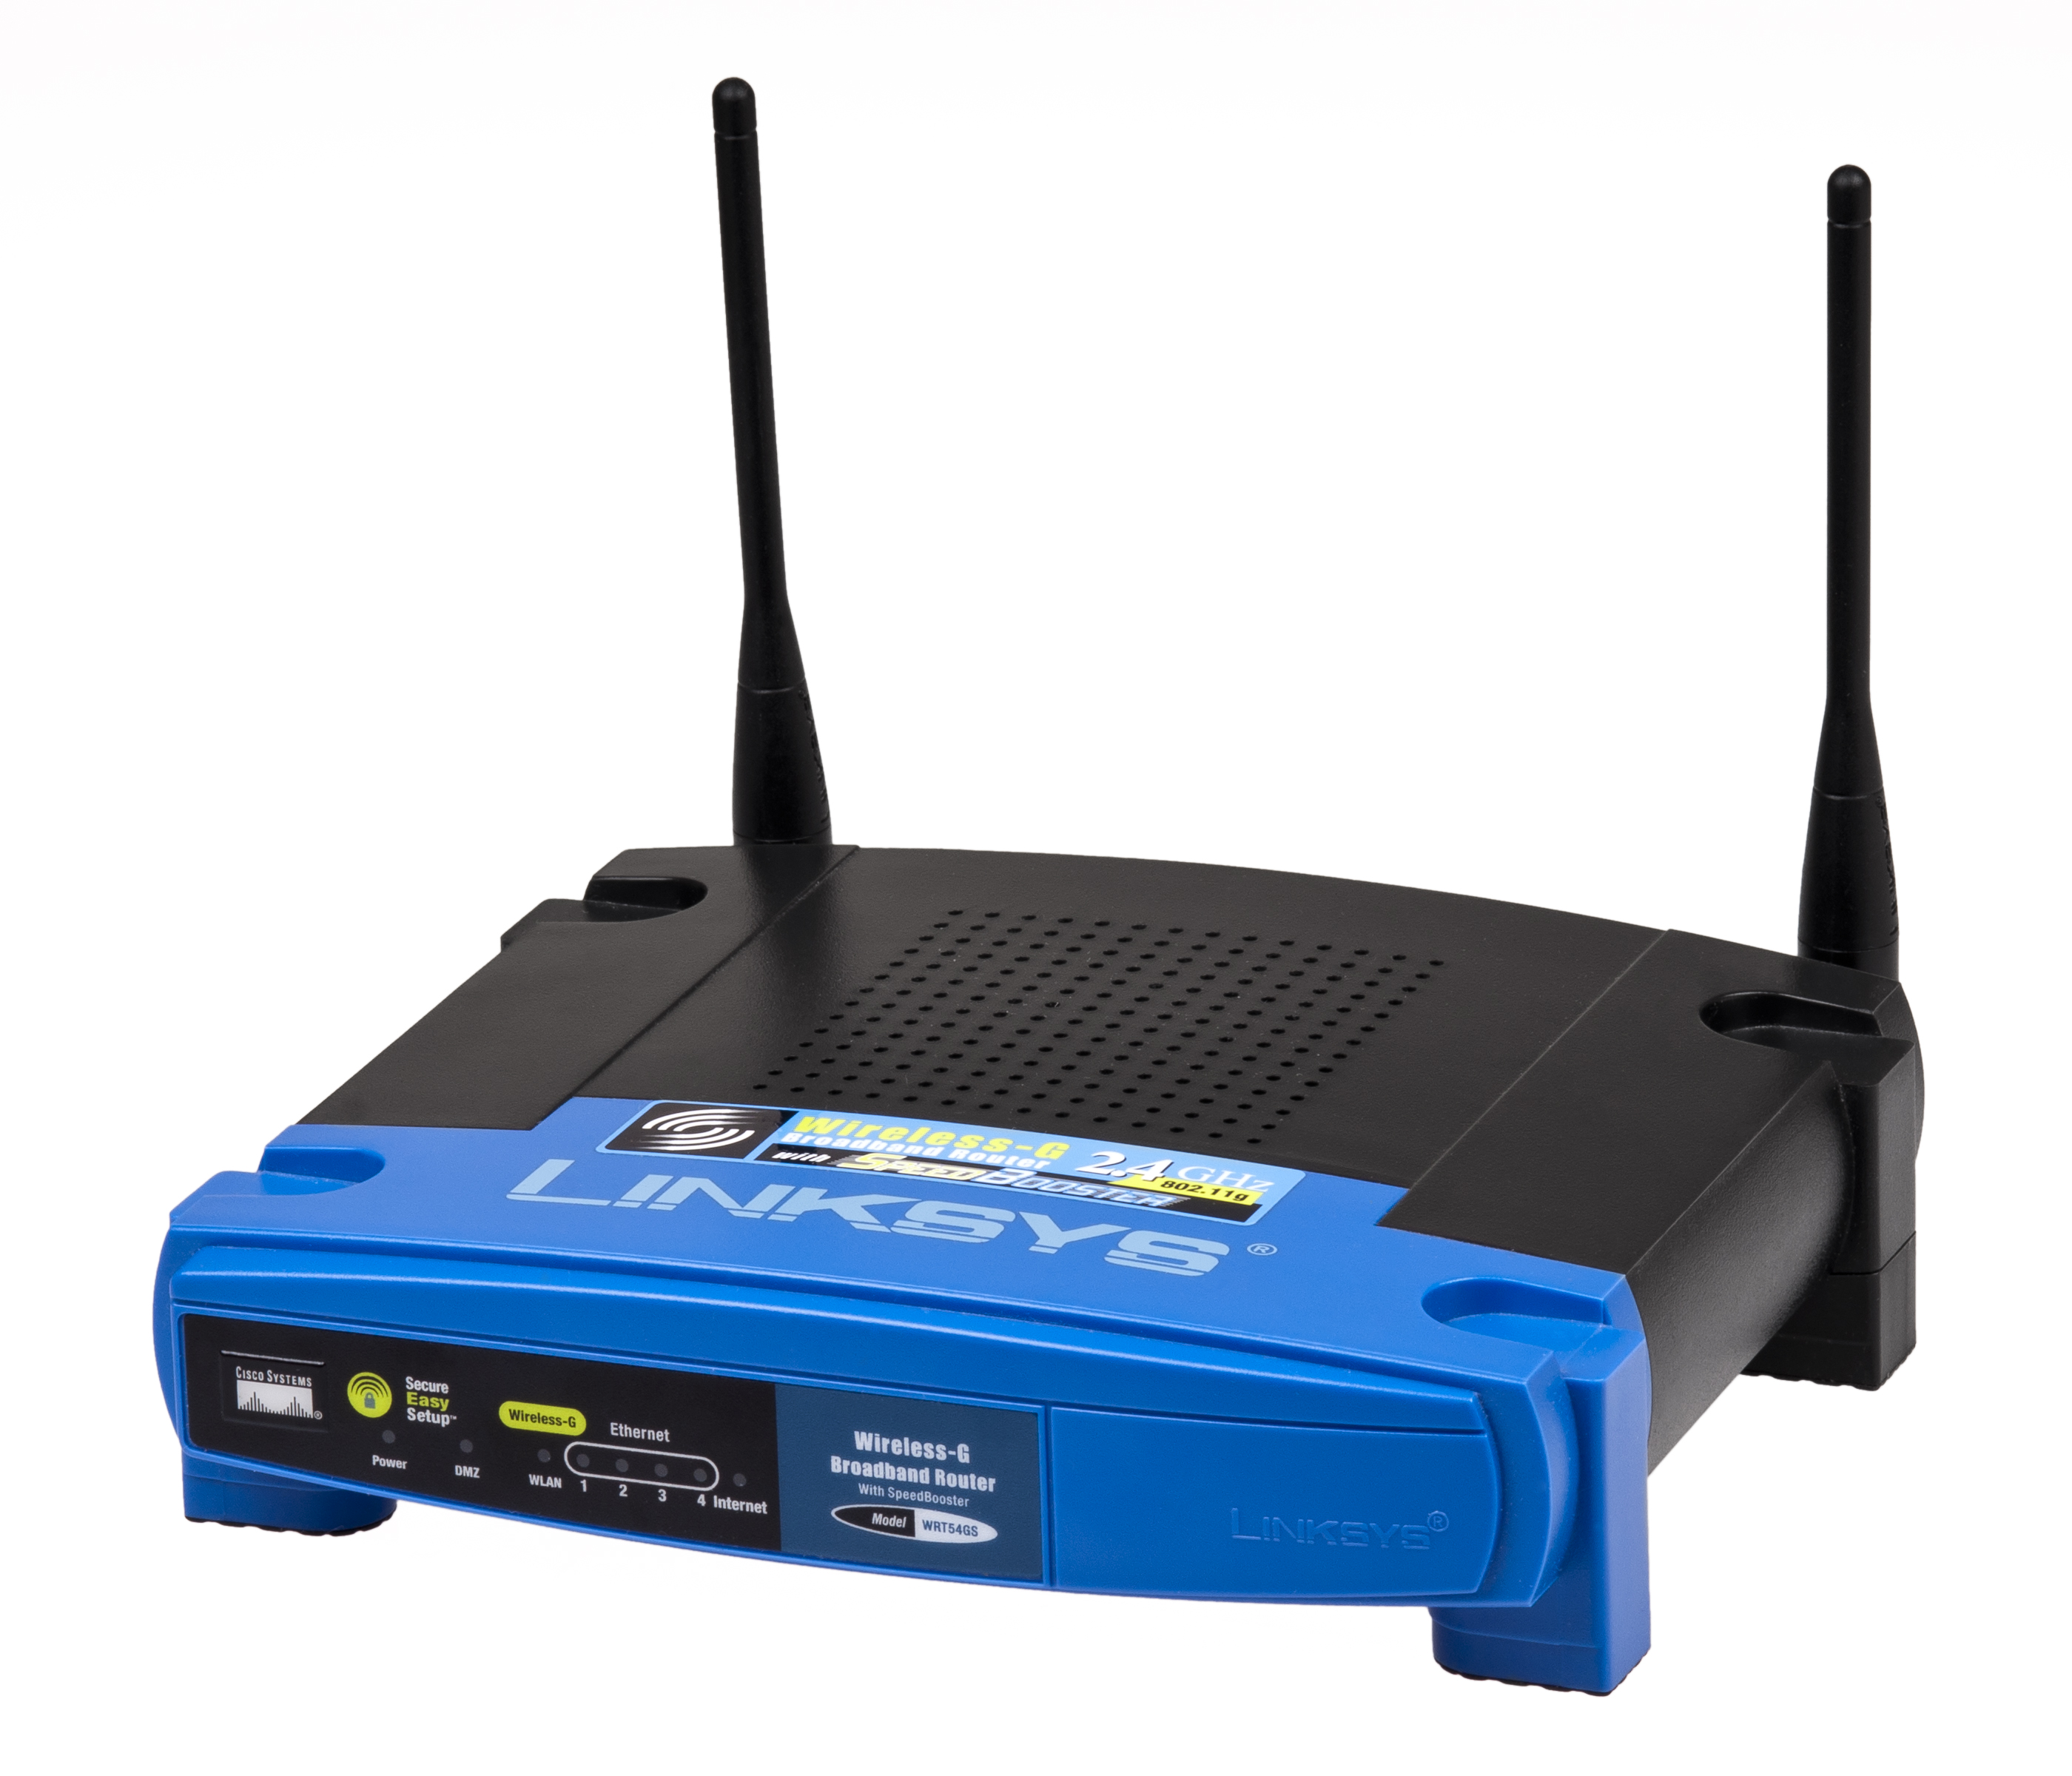
\includegraphics[height=2.5cm]{pictures/router.jpg}
  \end{tabular}
\end{frame}

\begin{frame}{Systèmes embarqués GNU/Linux?}
  \begin{itemize}
  \item Utilisé depuis longtemps comme serveur
  \item Pourquoi ne pas l'utiliser pour d'autres systèmes génériques?
  \item De nombreuses architectures supportées par Linux (ARM, mips, powerpc ...)
  \item Systèmes fiables et performants
  \item De nombreuses fonctionnalités déjà codées et validées
  \item Nécessite un BSP (Board support package) et un peu d'adaptation
  \end{itemize}
\end{frame}

\subsection{Eléments nécéssaires}
\begin{frame}{Eléments nécéssaires}
  \begin{itemize}
  \item Une système GNU/Linux embarqué nécéssite:
    \begin{itemize}
    \item Chaîne de compilation croisée (Gcc, as, ld, LibC)
    \item Un Bootloader (U-Boot, barebox, grub, isolinux)
    \item Noyau Linux adapté à l'archi hardware
    \item Outils GNU/LINUX Commandes Linux (sh, ls, cp, etc.)
    \item Applications ...
    \item Outil de génération (BR, OE, ...)
    \end{itemize}
  \end{itemize}
\end{frame}

%%%%%%%%%%%%%%%%%%%%%%%%%%%%%%%%%%%%%%%%%%%%%%
\section{Toolchain}
%%%%%%%%%%%%%%%%%%%%%%%%%%%%%%%%%%%%%%%%%%%%%%

\begin{frame}{Toolchain}{}
  \begin{itemize}
  \item Un point très complexe !
  \item Nécessité de construire une chaîne croisée :
    \begin{itemize}
    \item GCC
    \item Binutils (as, ld, ...)
    \item Dépendances avec le noyau (system calls, ...) => erreur "Kernel too old"
    \item Choix d'une libC => Glibc, uClibc, Eglibc, ...
    \item GDB
    \item Toute autre bibliothèque utilisée => libstdc++
    \item Dépendances avec le compilateur hôte
    \end{itemize}
  \end{itemize}
\end{frame}

\begin{frame}{Toolchain}{}
  \begin{itemize}
  \item Interaction entre la libC et le noyau Linux
    \begin{itemize}
    \item Appels systèmes (nombre, définition)
    \item Constantes
    \item Structures de données, etc.
    \end{itemize}
  \item Compiler la libC – et certaines applications - nécessite les en-tête du noyau
  \item Disponibles dans <linux/...> et <asm/...> et d'autres répertoires des sources du noyau (include, ...)
  \end{itemize}
\end{frame}

\subsection{Compilateur binaire}
\begin{frame}{compilateur binaire}
  \begin{itemize}
  \item Utiliser un compilateur binaire :
    \begin{itemize}
    \item ELDK: http://www.denx.de/wiki/DULG/ELDK
    \item Code Sourcery : https://sourcery.mentor.com/sgpp/lite/arm/portal/release1803
    \item Bootlin's toolchains: https://toolchains.bootlin.com
    \item Installation simple
    \item Support (payant) possible
    \item Configuration connue => support par les forums
    \end{itemize}
  \item Par contre:
    \begin{itemize}
    \item Versions des composants figées
    \item Non utilisation des possibilitées du CPU
    \item Choix libC limité
    \end{itemize}
  \end{itemize}
\end{frame}

\subsection{Compilateur source}
\begin{frame}{Compilé son compilateur}
  \begin{itemize}
  \item Construire un compilateur:
    \begin{itemize}
    \item Crosstool => obsolète
    \item Crosstool-NG => assez complexe à prendre en main
    \item Buildroot / OpenEmbedded
    \end{itemize}
  \item Aucun n'est "plug and play"
  \item La mise au point peut prendre des jours, voire plus !
  \item Binaires produits : arm-linux-* (gcc, as, ld, ar, nm, ...)
  \end{itemize}
\end{frame}

%%%%%%%%%%%%%%%%%%%%%%%%%%%%%%%%%%%%%%%%%%%%%%
\section{Construire son système embarqué}
%%%%%%%%%%%%%%%%%%%%%%%%%%%%%%%%%%%%%%%%%%%%%%

\subsection{Bootloader}
\begin{frame}{Bootloader}{}
  \begin{itemize}
  \item Premier logiciel lancé au démarrage de la machine
  \item Initialise le matériel (RAM, stockage, ...) nécésaire au boot
  \item Charge le noyau en RAM et lui donne la main
  \item Permet de donner des arguments au noyau
  \item Exemples:
    \begin{itemize}
    \item U-boot (supporte de nombreux architectures, la référence)
    \item Barebox (u-boot v2, meilleure archi, moins de fonctionnalités pour l'instant)
    \item grub (x86, serveur et desktop principalement)
    \item isolinux (alternative x86 à grub)
    \end{itemize}
  \item Un système embarqué nécéssitera une configuration et un support matériel dans le bootloader.
  \end{itemize}
\end{frame}

\subsection{Kernel}
\begin{frame}{Kernel}{}
  \begin{itemize}
  \item Génération d'un noyau:
    \begin{enumerate}
    \item Récupération du noyau (kernel.org)
    \item Développement du support des drivers manquants
    \item Création du support de la carte (board config  3.10 device tree)
    \item Configuration le noyau (make menuconfig)
    \item Compilation du noyau (make uImage)
    \item Installation sur la cible
    \end{enumerate}
  \item Binaire utilisable dans arch/arm/boot/zImage ou bien arch/arm/boot/uImage (pour U-Boot)
  \item Binaire vmlinux utile pour le debug
  \item Utilisation des variables ARCH et CROSS\_COMPILE.
  \end{itemize}
\end{frame}

\subsection{Rootfs}
\begin{frame}{Binaires de base}{}
  \begin{itemize}
  \item Binaires de base indispensables au système (ls, bash, dd, top, cp, mv, init,...)
  \item Trois possibilités:
    \begin{itemize}
    \item Récupérer les sources et les compiler un par un. (laborieux)
    \item GNU/Linux coreutils (trop lourd pour l'embarqué)
    \item Busybox (regroupe la majorité des commandes Linux en un seul executable)
      \begin{itemize}
      \item 95\% des distributions Linux embarqués l'utilise
      \item Simple, léger, portable
      \item Diffusé sous licence GPLv2
      \end{itemize}
    \end{itemize}
  \end{itemize}
\end{frame}

\begin{frame}{Busybox}{}
  \begin{itemize}
  \item Utilisation des variables ARCH et CROSS\_COMPILE. (comme le noyau)
  \item Génération de busybox:
    \begin{enumerate}
    \item Récupération des sources
    \item Configuration (make menuconfig)
    \item Compilation (make uImage)
    \item Installation sur la cible (make CONFIG\_PREFIX=... install)
    \end{enumerate}
  \end{itemize}
\end{frame}

\begin{frame}{Rootfs - Peuplement}
  \begin{itemize}
  \item Peuplement d'un rootfs:
    \begin{enumerate}
    \item Installation de la libc et des autres librairies fournies par la toolchain
    \item Installation des binaires de busybox
    \item Création de la configuration de démarrage (/etc/init.d)
    \item Ajout des nodes dans /dev (si pas de mécanisme automatique)
    \item Ajout des librairies et applications du projet.
    \end{enumerate}
  \item Deux mèthodes:
    \begin{itemize}
    \item A la main, copier ou installer chaque fichier/logiciel manuellement. (LFS) => Inenvisageable à moyen et long terme
    \item Automatiser soit en scriptant soit en utilisant un système existant (OE, yocto, buildroot, uclinux ...) => Plus rapide et plus sure. Indispensable en production pour maitriser son livrable.
    \end{itemize}
  \end{itemize}
\end{frame}

%%%%%%%%%%%%%%%%%%%%%%%%%%%%%%%%%%%%%%%%%%%%%%
\section{Mise au point}
%%%%%%%%%%%%%%%%%%%%%%%%%%%%%%%%%%%%%%%%%%%%%%

\subsection{BSP}
\begin{frame}{BSP}{}
  \begin{itemize}
  \item Une plateforme "neuve" nécéssite des ajustements pou fonctionner:
    \begin{itemize}
    \item Adaptation de la toolchain
    \item Support des drivers dans le \textbf{bootloader} et le \textbf{kernel}
    \item Ajout des fonctionnalités dans le bootloader et le kernel (réseau, NAND, HDD, ...)
    \end{itemize}
  \item Fourni par le constructeur de la plateforme éléctronique.
  \item Si on est le constructeur, il faut développer le support.
  \item Outils à disposition (gdb, sonde JTAG, ftrace, oscilloscope, multimetre ...)
  \end{itemize}
\end{frame}

\subsection{User space}
\begin{frame}{User space}{}
  \begin{itemize}
  \item Lorsque le BSP est OK, la mise au point en espace utilisateur peut commencer
  \item De nombreux outils permettent de mettre au point des applications:
    \begin{itemize}
    \item printf: outil simple à mettre en oeuvre et connu de tout le monde
    \item syslog: utile pour vérifier le bon fonctionnement ou detecter des anomalies
    \item valgrind: vérifie la bonne utilisation de la mémoire
    \item strace/ltrace: affiche les appels systèmes et librairies
    \item gdb: debugguer GNU/LINUX
      \begin{itemize}
      \item permet d'acceder à la memoire, controler l'execution, monitoré les threads ...
      \item gdbserver pour les cibles embarqués pour déporter le debug
      \end{itemize}
    \end{itemize}
  \end{itemize}
\end{frame}
